\chapter{Organisation}

\section{Planning et répartition du travail}

En raison de l'abandon du projet par Thibaud LE DOLEDEC et Clément AILLOUD partis en stage, le projet ne pourra être mené à terme. Pour aborder la dernière ligne droite avant l'évaluation finale, un choix a donc été fait des tâches sur lesquelles travailler en priorité, au détriment d'autres qui demeureront inachevées.

\vspace{1cm}

Ci-dessous un diagramme représentant l’avancement des différentes tâches du projet. Le gris indique qu’une tâche est terminée ou à un niveau d’avancement satisfaisant et garantissant une maturité proche. Le orange indique les tâches en cours ou prioritaires au moment de l'évaluation finale. Les flèches représentent des liens de dépendance entre certaines tâches.

\begin{figure}[H]
    \centering
	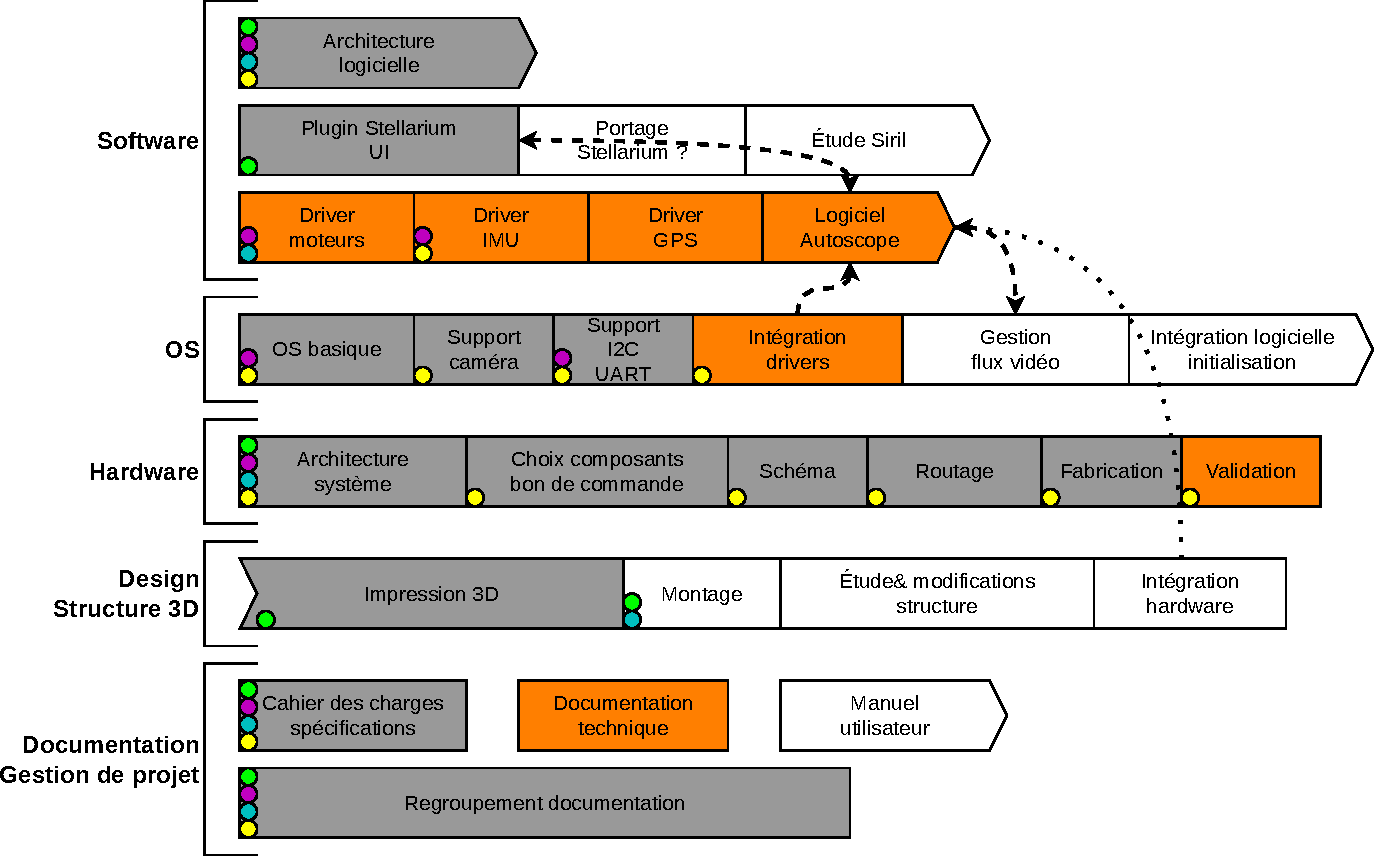
\includegraphics[width=1\linewidth]{\figures/sch_gantt.pdf}
    \decoRule
    \caption[
    Diagramme de l'organisation temporelle du travail sur le projet]{
    Diagramme de l'organisation temporelle du travail sur le projet}
    \label{fig:Diagramme de l'organisation temporelle du travail sur le projet}
    \end{figure}


\section{Accessibilité du projet sur internet}

Le projet étant libre, il est disponible sur Github sous licence GPL-2. Nous tachons d'accompagner nos différents dépôts d'une documentation claire permettant d'obtenir les informations suivantes~:
\begin{itemize}[label=$\bullet$]
	\item Une description brève et précise sur le contenu du dépôt et son rôle au sein du projet.
	\item Une explication de la procédure à suivre pour utiliser le contenu du dépôt.
	\item Une explication de la procédure à suivre pour travailler sur le dépôt.
	\end{itemize}

\subsection{Dépôt principal}

{\href{https://github.com/thibaudledo/Autoscope}{\codeinline{text}{https://github.com/thibaudledo/Autoscope}}}

\vspace{1cm}

Le dépôt est organisé comme suit~:
\begin{itemize}[label=$\bullet$]
	\item Branche {\href{https://github.com/thibaudledo/Autoscope/tree/master}{\codeinline{text}{master}}}~: Sources du logiciel principal et explications sur le projet dans son ensemble.
	\item Release {\href{https://github.com/thibaudledo/Autoscope/releases}{\codeinline{text}{alpha}}}~: Paquets et fichiers binaires pour utiliser le projet "out of the box" (release expérimentale).
	\item Branche {\href{https://github.com/thibaudledo/Autoscope/tree/hardware}{\codeinline{text}{hardware}}}~: Fichiers Blender de la structure du télescope et fichiers KiCad de la carte électronique du projet.
	\item Branche {\href{https://github.com/thibaudledo/Autoscope/tree/doc}{\codeinline{text}{doc}}}~: Documentations et datasheets des composants et éléments utilisés pour le projet.
	\item Branche {\href{https://github.com/thibaudledo/Autoscope/tree/latex}{\codeinline{text}{latex}}}~: Fichiers LaTex et \codeinline{text}{.pdf} des comptes rendus sur le projet.
	\item Branche {\href{https://github.com/thibaudledo/Autoscope/tree/hello_mod}{\codeinline{text}{hello_mod}}}~: Sources d'un driver helloworld servant d'exemple.
	\item Branche {\href{https://github.com/thibaudledo/Autoscope/tree/a4988_mod}{\codeinline{text}{a4988_mod}}}~: Sources du driver des contrôleurs moteur et des capteurs de fin de course des moteurs.
	\item Branche {\href{https://github.com/thibaudledo/Autoscope/tree/mpu9250_mod}{\codeinline{text}{mpu9250_mod}}}~: Sources du driver de la centrale inertielle.
	\item Branche {\href{https://github.com/thibaudledo/Autoscope/tree/mtk3339d}{\codeinline{text}{mtk3339d}}}~: Sources du driver du GPS.
	\end{itemize}

\newpage
\subsection{Dépôt du système d'exploitation de la Raspberry-Pi}

{\href{https://github.com/thomaslepoix/meta-autoscope}{\codeinline{text}{https://github.com/thomaslepoix/meta-autoscope}}}

\vspace{1cm}

Il s'agit de la couche de métadonnées utilisées par Yocto pour construire le système d'exploitation Linux utilisé par la Raspberry-Pi du télescope. Une image pré-compilée du système d'exploitation figurera sur {\href{https://github.com/thibaudledo/Autoscope/releases}{la release \codeinline{text}{alpha} du dépôt principal}.

\vspace{1cm}

Le dépôt est organisé comme suit~:
\begin{itemize}[label=$\bullet$]
	\item Branche {\href{https://github.com/thomaslepoix/meta-autoscope/tree/rpi}{\codeinline{text}{rpi}}}~: Métadonnées Yocto et explications de comment compiler et installer le système d'exploitation.
	\item Branche {\href{https://github.com/thomaslepoix/meta-autoscope/tree/rpi-repo}{\codeinline{text}{rpi-repo}}}~: Données utilisées par Repo pour synchroniser le dépôt à d'autres dépôts de métadonnées Yocto utilisées pout construire l'OS.
	\end{itemize}

\subsection{Dépôt du plugin de Stellarium}

{\href{https://github.com/thibaudledo/Autoscope-Stellarium-plugin}{\codeinline{text}{https://github.com/thibaudledo/Autoscope-Stellarium-plugin}}}

\vspace{1cm}

Il s'agit du plugin de Stellarium contenant l'interface par laquelle l'utilisateur interagira avec le télescope. Un paquet pré-compilé pour linux de Stellarium incluant le plugin figure sur {\href{https://github.com/thibaudledo/Autoscope/releases}{la release \codeinline{text}{alpha} du dépôt principal}.

\vspace{1cm}

Le dépôt est organisé comme suit~:
\begin{itemize}[label=$\bullet$]
	\item Branche {\href{https://github.com/thibaudledo/Autoscope-Stellarium-plugin/tree/master}{\codeinline{text}{master}}}~: Sources du plugin, patch des sources de Stellarium et explications de comment compiler une version de Stellarium intégrant le plugin.
	\end{itemize}

